\documentclass[a4paper,11pt]{article}

\usepackage[english]{babel}
\usepackage{float}
\usepackage{graphicx}
\usepackage{amsmath,amsthm}
\usepackage{gensymb}
\usepackage{amssymb}
\usepackage[margin=2.cm]{geometry}
\usepackage{pstricks-add}	%for geometric diagrams
\usepackage{chemfig}	%for structural formulae
\usepackage{tabularx}	%for better tables
\usepackage{booktabs}	%for better tables
\usepackage[makeroom]{cancel}	%for cancelling lines
\usepackage{hyperref}	%hyperlinks
\usepackage{mathrsfs}
\usepackage{mathtools}
\usepackage{epigraph}	%quotes
\usepackage{lastpage}
\usepackage{multicol}	%column environments
\usepackage{fancyhdr}	%headers
\usepackage[at]{easylist}	%easy lists
\usepackage{wasysym}
\usepackage{wrapfig}	%wrap figures in text
\usepackage{subfig}		%subfigures
\usepackage{tikz}

\allowdisplaybreaks
\newcommand\numberthis{\addtocounter{equation}{1}\tag{\theequation}}
\setlength{\epigraphwidth}{7.7cm}
\setlength{\tabcolsep}{10pt}

% bracket group shorthands
\newcommand{\abs}[1]{\left|#1\right|}
\newcommand{\set}[1]{\left\{#1\right\}}

% common sets
\newcommand{\R}{\mathbb{R}}
\newcommand{\Cmplx}{\mathbb{C}}
\newcommand{\Q}{\mathbb{Q}}
\newcommand{\Z}{\mathbb{Z}}
\newcommand{\N}{\mathbb{N}}

% derivative shorthands
\newcommand{\diff}[2]{\frac{\mathrm{d}#1}{\mathrm{d}#2}}
\newcommand{\pdiff}[2]{\frac{\partial #1}{\partial #2}}
\newcommand{\ndiff}[3]{\frac{\mathrm{d}^{#3}#1}{\mathrm{d}#2^{#3}}}
\newcommand{\npdiff}[3]{\frac{\partial^{#3} #1}{\partial #2^{#3}}}

% theorem environments
\newtheorem*{definition*}{Definition}
\newtheorem*{lemma*}{Lemma}
\newtheorem{theorem}{Theorem}
\newtheorem*{theorem*}{Theorem}
\newtheorem*{corollary*}{Corollary}
\newtheorem{example}{Example}
\newtheorem*{remark}{Remark}

\DeclareMathOperator{\bdy}{Bdy}
\DeclareMathOperator{\interior}{Int}

% header
\pagestyle{fancy}
\lhead{Problem Set 2}
\rhead{Year 11 2018}

%\title{Problem Set 2}
%\date{\today}
%\author{Daniel Czapski}

\begin{document}
	\section*{Essential Revision Problems -- Set 2 -- Locus and Parametrics, Combinatorics and Probability, and Polynomials}
	\subsection*{Question 1: 2001 Q6 b.}
	Consider the point $P(2at,at^2)$ on the parabola $x^2=4ay$.\\
    
	\begin{easylist}[enumerate]
		\ListProperties(Numbers1=r,Numbers2=a,Progressive=1cm,Margin1=1cm,FinalMark={)},Space*=0.5cm)
		@ Prove that the equation of the normal at $P$ is $x+ty=2at+at^3$.
        @ Find the coordinates of the point $Q$ on the parabola such that the normal at $Q$ is perpendicular to the normal at $P$.
        @ Show that the two normals of part ii) intersect at the point $R$ with coordinates 
        \begin{align*}
        x = a\left(t-\frac{1}{t}\right) && y = a\left(t^2+1+\frac{1}{t^2}\right).
        \end{align*}
        @ Find the Cartesian form of the equation of the locus of the point $R$.
	\end{easylist}
    
    \subsection*{Question 2: CBHS Lewisham 2014 Preliminary Final}
    Show that if $y=mx+b$ is a tangent to the curve $x^2=4ay$ then $am^2+b=0$.\\
    
    \noindent (Yes, I still have my old preliminary exams lying around)
    
    \subsection*{Question 3: 2014 Q13 c.}
    The point $P(2at,at^2)$ lies on the parabola $x^2=4ay$ with focus $S$. The point $Q$ divides the interval $PS$ internally in the ratio $t^2:1$.\\
    
	\begin{easylist}[enumerate]
		\ListProperties(Numbers1=r,Numbers2=a,Progressive=1cm,Margin1=1cm,FinalMark={)},Space*=0.5cm)
		@ Show that the coordinates of the point $Q$ are given by 
        \begin{align*}
        x=\frac{2at}{1+t^2} && y=\frac{2at^2}{1+t^2}.
        \end{align*}
        @ Express the slope of $OQ$ in terms of $t$.
        @ Using the result from part ii), or otherwise, show that $Q$ lies on a fixed circle of radius $a$.
	\end{easylist}
    \pagebreak

% \subsection*{Question 4: Inspired by my morning commute}
% It is well known by frequent users of public transport that every carriage on a Sydney Trains train has a four digit serial number comprised of digits between 0 and 9 (inclusive!). The ``Train Game'' (or whatever students call it now) has the simple aim of combining the digits of the carriage serial number, using standard operations, to make ten\footnote{Sometimes this is very easy; other times this is particularly difficult and sometimes it is impossible! An interesting problem to consider is this: what conditions must be imposed on a serial number in order to guarantee that there exists at least one way to make ten?}. Traditionally, it is stipulated that no number can be used more than once and all numbers must be used in the order in which they appear. For example, 1345: $(1-3+4)\times5$.\\

% \noindent I'm bad at basic arithmetic and my morning train ride isn't that long, so I prefer to rearrange the numbers into whatever order is convenient. Thus, suppose the order of the digits is NOT important (i.e. 1234 and 3421 are equivalent). \\
% 	\begin{easylist}[enumerate]
% 		\ListProperties(Numbers1=r,Numbers2=r,Progressive=1cm,Margin1=1cm,FinalMark={)},Space*=0.5cm)
% 		@ If serial numbers have no repetitions, how many different serial numbers are possible?
%         @ Serial numbers often DO have repetitions. If we permit this, how many are possible?
%         @ Repeat parts i) and ii), but for five digit serial numbers.
%     \end{easylist}
%     \vspace{0.5cm}
% \noindent Suppose we insist that we use the numbers in order. That is, order is important (i.e. 1234 and 3421 are NOT equivalent). \\
% 	\begin{easylist}[enumerate]
% 		\ListProperties(Start1=4,Numbers1=r,Numbers2=r,Progressive=1cm,Margin1=1cm,FinalMark={)},Space*=0.5cm)
% 		@ Repeat parts i), ii) and iii) assuming order is important.
%     \end{easylist}

\subsection*{Question 4: Inspired by my morning commute}
It is well known by frequent users of public transport that every carriage on a Sydney Trains train has a four digit serial number comprised of digits between 0 and 9 (inclusive!). The ``Train Game'' (or whatever students call it now) has the simple aim of combining the digits of the carriage serial number, using standard operations, to make ten\footnote{Sometimes this is very easy; other times this is particularly difficult and sometimes it is impossible! An interesting problem to consider is this: what conditions must be imposed on a serial number in order to guarantee that there exists at least one way to make ten?}. Traditionally, it is stipulated that no number can be used more than once and all numbers must be used in the order in which they appear. For example, 1345: $(1-3+4)\times5$.\\

\noindent I'm bad at basic arithmetic and my morning train ride isn't that long, so I prefer to rearrange the numbers into whatever order is convenient. Thus, suppose the order of the digits is NOT important (i.e. 1234 and 3421 are equivalent). \\
	\begin{easylist}[enumerate]
		\ListProperties(Numbers1=r,Numbers2=r,Progressive=1cm,Margin1=1cm,FinalMark={)},Space*=0.5cm)
		@ If serial numbers have no repetitions, how many different serial numbers are possible?
    \end{easylist}
    \vspace{0.5cm}
    \noindent Serial numbers often DO have repeats, however. For example, a three digit serial number could comprise a triple (e.g. 111), a pair and a single (e.g. 112) or three singles (e.g. 123); there are three unique cases to consider.\\
	\begin{easylist}[enumerate]
		\ListProperties(Start1=2,Numbers1=r,Numbers2=r,Progressive=1cm,Margin1=1cm,FinalMark={)},Space*=0.5cm)
        @ For a four digit serial number, how many unique cases are there? List them.
        @ How many different arrangements are possible, assuming order is unimportant (i.e. 1234 and 3421 are considered the same, as they both comprise 1, 2, 3 and 4) and repetitions are permitted?
        @ Repeat parts i), ii) and iii), but for five digit serial numbers.
    \end{easylist}
    \vspace{0.5cm}
\noindent Suppose we insist that we use the numbers in order. That is, order is important (i.e. 1234 and 3421 are NOT equivalent). \\
	\begin{easylist}[enumerate]
		\ListProperties(Start1=5,Numbers1=r,Numbers2=r,Progressive=1cm,Margin1=1cm,FinalMark={)},Space*=0.5cm)
		@ Repeat parts i), ii), iii) and iv) assuming order is important.
    \end{easylist}
    
% I reckon this question is quite challenging! I'm very interested to see what solutions are devised.

\subsection*{Question 5: 2009 Q6 c.}
Consider a square grid with $n$ rows and $n$ columns of equally spaced points.

\begin{center}
	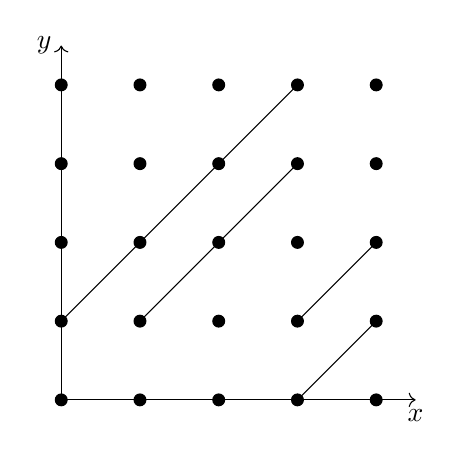
\begin{tikzpicture}
	\draw[->] (0,0) -- (4.5,0) node[below] {$x$};
    \draw[->] (0,0) -- (0,4.5) node[left] {$y$};
    \foreach \x in {0,...,4} {
    	\foreach \y in {0,...,4} {
        	\draw[fill=black] (\x,\y) circle[radius=0.075cm];
        }
    }
    
    \draw (3,0) -- (4,1);
    \draw (3,1) -- (4,2);
    \draw (1,1) -- (3,3);
    \draw (0,1) -- (3,4);
	\end{tikzpicture}
\end{center}
The diagram illustrates such a grid. Several intervals of gradient 1, whose endpoints are a pair of points in the grid, are shown. 
\pagebreak
\vspace{0.15cm}
	\begin{easylist}[enumerate]
		\ListProperties(Numbers1=r,Numbers2=r,Progressive=1cm,Margin1=1cm,FinalMark={)},Space*=0.5cm)
		@ Explain why the number of such intervals on the line $y=x$ is equal to $\binom{n}{2}$.
        @ Explain why the total number, $S_n$, of such intervals in the grid is given by 
        $$
        S_n = \binom{2}{2} + \binom{3}{2} + \cdots + \binom{n-1}{2} + \binom{n}{2} + \binom{n-1}{2} + \cdots + \binom{3}{2} + \binom{2}{2}.
        $$
        @ Given 
        $$
        \binom{n+1}{r+1} = \binom{r}{r} + \binom{r+1}{r} + \cdots + \binom{n}{r}
        $$
        show that 
        $$
        S_n = \frac{n(n-1)(2n-1)}{6}.
        $$
    \end{easylist}
    
    \subsection*{Question 6: 2006 Q6 b.}
    In an endurance event, the probability that a competitor will complete the course is $p$ and the probability that a competitor will not complete the course is $q=1-p$. Teams consist of either two or four competitors. A team scores points if at least half its members complete the course.\\
    
	\begin{easylist}[enumerate]
		\ListProperties(Numbers1=r,Numbers2=r,Progressive=1cm,Margin1=1cm,FinalMark={)},Space*=0.5cm)
		@ Show that the probability that a four-member team will have at least three of its members not complete the course is $4pq^3+q^4$.
        @ Hence, or otherwise, find an expression in terms of $q$ only for the probability that a four-member team will score points.
        @ Find an expression in terms of $q$ only for the probability that a two-member team will score points.
        @ Hence, or otherwise, find the range of values of $q$ for which a two-member team is more likely than a four-member team to score points.
    \end{easylist}
    
    \subsection*{Question 7: 1990 (4U) Q6 a.}
	\begin{easylist}[enumerate]
		\ListProperties(Numbers1=r,Numbers2=r,Progressive=1cm,Margin1=1cm,FinalMark={)},Space*=0.5cm)
		@ Write down the relations which hold between the roots $\alpha,\beta$ and $\gamma$ of the equation $ax^3+bx^2+cx+d=0,a\neq0$ and the coefficients $a,b,c$ and $d$.
        @ Consider the equation $36x^3-12x^2-11x+2=0$. You are given that the roots $\alpha, \beta$ and $\gamma$ of this equation satisfy $\alpha=\beta+\gamma$. Use part i) to find $\alpha$. 
        @ Suppose that the equation $x^3+px^2+qx+r=0$ has roots $\lambda, \mu$ and $\nu$ which satisfy $\lambda=\mu+\nu$. Show that $p^3-4pq+8r=0$.
    \end{easylist}
\end{document}